%-------------------------------------------------------------------------------
% This file provides a skeleton ATLAS paper.
%-------------------------------------------------------------------------------
% \pdfoutput=1
% The \pdfoutput command is needed by arXiv/JHEP/JINST to ensure use of pdflatex.
% It should be included in the first 5 lines of the file.
\pdfinclusioncopyfonts=1
% This command may be needed in order to get \ell in PDF plots to appear. Found in
% https://tex.stackexchange.com/questions/322010/pdflatex-glyph-undefined-symbols-disappear-from-included-pdf

% Specify where ATLAS LaTeX style files can be found.
\RequirePackage{latex/atlaslatexpath}
% Comment out the above line if the files are in a central location, e.g. $HOME/texmf.
%-------------------------------------------------------------------------------
\documentclass[NOTE, REPORT=true, atlasdraft=true, USenglish]{atlasdoc}

\usepackage[hyphens,spaces,obeyspaces]{url}
\usepackage{pgfplots}
\usepackage{subcaption}
\pgfplotsset{width=10cm,compat=1.9}
\usepackage{graphicx}
\usepackage{amsmath}  % For advanced math symbols
\usepackage[version=4]{mhchem}   % For units like GeV
\graphicspath{ {./images/} }
\usepackage{atlaspackage}
% Style file with biblatex options for ATLAS documents.
\usepackage{atlasbiblatex}
% Useful macros
\usepackage{atlasphysics}
% See doc/atlas_physics.pdf for a list of the defined symbols.
% This package should not be used in the final version of the paper.
\ifthenelse{\boolean{AtlasDraft}}{\usepackage[output=true, shift=true]{atlastodo}}{}
% Files with references for use with biblatex.
% Note that biber gives an error if it finds empty bib files.
\addbibresource{mydocument.bib}
% Paths for figures - do not forget the / at the end of the directory name.
\graphicspath{{logos/}{figures/}}
% Add your own definitions here (file mydocument-defs.sty).
\usepackage{mydocument-defs}
\usepackage{listings}
\usepackage{xcolor}

%New colors defined below
\definecolor{codegreen}{rgb}{0,0.6,0}
\definecolor{codegray}{rgb}{0.5,0.5,0.5}
\definecolor{codepurple}{rgb}{0.58,0,0.82}
\definecolor{backcolour}{rgb}{0.95,0.95,0.92}

%Code listing style named "mystyle"
\lstdefinestyle{mystyle}{
  backgroundcolor=\color{backcolour}, commentstyle=\color{codegreen},
  keywordstyle=\color{magenta},
  numberstyle=\tiny\color{codegray},
  stringstyle=\color{codepurple},
  basicstyle=\ttfamily\footnotesize,
  breakatwhitespace=false,         
  breaklines=true,                 
  captionpos=b,                    
  keepspaces=true,                 
  numbers=left,                    
  numbersep=5pt,                  
  showspaces=false,                
  showstringspaces=false,
  showtabs=false,                  
  tabsize=2
}

%program names
\newcommand{\Py}{\tsc{Pythia}}


%-------------------------------------------------------------------------------
% Generic document information.
%-------------------------------------------------------------------------------

% Title, abstract and document.
%-------------------------------------------------------------------------------
% This file contains the title, author and abstract.
% It also contains all relevant document numbers used by the different cover pages.
%-------------------------------------------------------------------------------

% Title
\AtlasTitle{AQP: Deployment of Delta-matching in MG3.5.0}

% Draft version:
% Should be 1.0 for the first circulation, and 2.0 for the second circulation.
% If given, adds draft version on front page, a 'DRAFT' box on top of every other page, 
% and line numbers.
% Comment or remove in the final version.
\AtlasVersion{0.1}

% Abstract - % directly after { is important for correct indentation
\AtlasAbstract{%
  This is a bare bones ATLAS document. Put the abstract for the document here.
}

% Author - this does not work with revtex (add it after \begin{document})
% This has to be commented out for TDR etc.
% For PUB notes, add package authblk and use \thanks if an ACE/STA should be added.
% See Section 4.2 of ATLAS LaTeX guide and latex/atlascontribute.sty for more details.
\author{Dongyi Liu}

% ATLAS reference code, to help ATLAS members to locate the paper
\AtlasRefCode{GROUP-2024-XX}

% CERN preprint number
% \PreprintIdNumber{CERN-EP-2024-XX}

% ATLAS date - arXiv submission; usually filled in by the Physics Office
% \AtlasDate{\today}

% ATLAS heading - heading at top of title page. Set for TDR etc.
% \AtlasHeading{ATLAS ABC TDR}

% Keywords - some journals want keywords on the title page.
% You have to pass the option keywords=true to atlasdoc for this to be effective.
% \AtlasKeywords{keywords}

% Copyright - use if something other than the default copyright is required.
% You have to pass the option copyright=true to atlasdoc for this to be effective.
% \AtlasCopyright{\the\year \ CERN for the benefit of the ATLAS Collaboration.\newline
%   Reproduction of this article or parts of it is allowed as specified in the CC-BY-4.0 license.}

% arXiv identifier
% \arXivId{21XX.YYYY}

% HepData record
% \HepDataRecord{ZZZZZZZZ}

% Submission journal and final reference
% \AtlasJournal{Phys.\ Lett.\ B.}
% \AtlasJournalRef{\PLB 789 (2023) 123}
% \AtlasDOI{}

% Some papers/public notes have a special author list.
% If a special author list should be indicated via a link use the following code:
% Include the two lines below if you do not use atlasstyle:
% \usepackage[marginal,hang]{footmisc}
% \setlength{\footnotemargin}{0.5em}
% Use the following lines in all cases:
% \usepackage{authblk}
%\author{The ATLAS Collaboration}
% \thanks{The full author list can be found at:\newline
%   \url{https://atlas.web.cern.ch/Atlas/PUBNOTES/ATL-PHYS-PUB-2024-XXX/authorlist.pdf}}
% }
% You may need the following lines if the affiliation number does not appear as a superscript
% when you are using authblk.
% \makeatletter
% \renewcommand\AB@authnote[1]{{\normalfont\textsuperscript{#1}}}
% \renewcommand\AB@affilnote[1]{{\normalfont\textsuperscript{#1}}}
% \makeatother

%-------------------------------------------------------------------------------
% The following information is needed for the cover page. The commands are defined
% if you use the coverpage option in atlasdoc or use the atlascover package.
% They are also defined if you include the atlasmetadefs package.
%-------------------------------------------------------------------------------

% List of supporting notes  (leave as null \AtlasCoverSupportingNote{} if you want to skip this option)
% \AtlasCoverSupportingNote{Short title note 1}{https://cds.cern.ch/record/XXXXXXX}
% \AtlasCoverSupportingNote{Short title note 2}{https://cds.cern.ch/record/YYYYYYY}
%
% OR (the 2nd option is deprecated, especially for CONF and PUB notes)
%
% Supporting material TWiki page  (leave as null \AtlasCoverTwikiURL{} if you want to skip this option)
% \AtlasCoverTwikiURL{https://twiki.cern.ch/twiki/bin/view/Atlas/WebHome}

% Comment deadline
% \AtlasCoverCommentsDeadline{DD Month 2024}

% Analysis team members - contact editors should no longer be specified
% as there is a generic email list name for the editors
% \AtlasCoverAnalysisTeam{Peter Analyser, Susan Editor1, Jenny Editor2, Alphonse Physicien}

% Editorial Board Members - indicate the Chair by a (chair) after his/her name
% Give either all members at once (then they appear on one line), or separately
% \AtlasCoverEdBoardMember{EdBoard~Chair~(chair), EB~Member~1, EB~Member~2, EB~Member~3}
% \AtlasCoverEdBoardMember{EdBoard~Chair~(chair)}
% \AtlasCoverEdBoardMember{EB~Member~1}
% \AtlasCoverEdBoardMember{EB~Member~2}
% \AtlasCoverEdBoardMember{EB~Member~3}

% A PUB note has readers and not an EdBoard -- give their names here (one line or several entries)
% \AtlasCoverReaderMember{Reader~1, Reader~2}
% \AtlasCoverReaderMember{Reader~1}
% \AtlasCoverReaderMember{Reader~2}

% Analysis team egroup
% \AtlasCoverEgroupAnalysisTeam{atlas-GROUP-2024-XX-analysis-team@cern.ch}

% EdBoard and conveners egroup
% \AtlasCoverEgroupEdBoard{atlas-GROUP-2024-XX-edboard-conveners@cern.ch}

% Author and title for the PDF file.
\hypersetup{pdftitle={ATLAS document},pdfauthor={Dongyi Liu}}

%-------------------------------------------------------------------------------
% Content
%-------------------------------------------------------------------------------
\begin{document}

\maketitle

\tableofcontents

% List of to-do notes.
% \listoftodos


\chapter{Introduction}
\label{chap:introduction}
%-------------------------------------------------------------------------------
%%%%%%%%%%%%%%%%%%%%%%%%% Physics background %%%%%%%%%%%%%%%%%%%%%%%%%%%%%
% 1. Why do we want to reduce negative weights fraction? What's the physics meaning of reducing it? What advantage we can gain from it? Why do we care about ttbar, tqZ, tW processes?





%%%%%%%%%%%%%%%%%%%%%%%%%  General overview of Monte Carlos event generator %%%%%%%%%%
% 1. What's Monte Carlo event generator for?
% 2. How does event generator work?
% 3. How many event generator does ATLAS have?
% 4. Why do we only use MG5 + Py8
According to perturbation theory, Monte Carlo event generators simulate collision events from the initial hard process to the long wavelengths of hadronization, and hadron decays to certain orders of accuracy. The main task of the MC event generator is to predict the cross-section of a given process with high precision. Matrix element (ME) calculations reduce uncertainties in the hard scattering regime, providing accurate simulation for high-energy interaction, and are usually implemented by \texttt{MadGraph5}. However, ME calculations become inefficient when dealing with collinear emissions of additional particles (like gluons) due to large infrared (IR) and collinear divergences. To handle soft and collinear radiation more effectively, parton showers are employed to model the subsequent evolution from hard scattering to the final states. Naturally, matrix element calculations should be combined with parton showers for a more comprehensive cross-section prediction, but this introduces the issue of double counting, which arises when the MC generates kinematical configurations with real parton emissions that are also included in the NLO computation, leading to discrepancies in predictions for any observable at the first order beyond the Born approximation, particularly in the soft and collinear regions where both MC and NLO results coincide for leading terms. The prescription of MC@NLO\cite{NLO_matching} in the framework of MadGraph5 addresses this by supporting both LO and NLO calculations\cite{MadGraph5}, using appropriate matching and merging schemes (e.g., MLM matching or FxFx merging\cite{merging}) to avoid double-counting when combining matrix elements and parton showers. However, this solution brings a new challenge: negative-weight events, which reduce the statistical power of the sample.


In recent years, it has become increasingly important to study the event-weight distribution directly, as generating large event samples can become computationally expensive. The presence of negative-weight event samples introduces higher variance in the calculated cross-section, which requires 3-5 times more events to achieve the same accuracy compared to a positive-definite simulation. Thus, reducing the Negative Weight Fraction (NWF) of events improves the computational efficiency as simulating these events consumes significant CPU time while diminishing the statistical power of the sample.


%1. What's the theoretical motivation for reducing negative weight fraction?
%2. How does delta matching strategy work?
%3. How does folding parameter work?

To mitigate the issue of negative-weight events, a new NLO-accurate matching prescription called MC@NLO-\text{$\Delta$}\cite{frederix_reduction_2020} was developed. This prescription starts with the MC@NLO cross section and augments it with additional elements from parton-shower MC simulations, with the ultimate goal of reducing the number of negative-weight events that are present in MC@NLO simulations. For the first time, we have achieved a practical implementation of the MC@NLO-$\Delta$ matching in ATLAS athena by including it in the \texttt{MADGRAPH5\_AMC@NLO} framework in conjunction with the \texttt{PYTHIA8} MC. Additionally, the folding technique used in \texttt{MADGRAPH5\_AMC@NLO} induces a further reduction of negative-weight events in both MC@NLO-$\Delta$ and MC@NLO. Folding parameters, which are user-tunable integers, control the density with which the phase space of the MC event generator is sampled during the integration process. A higher number of folding points leads to smoother distributions but also increases the computational cost, so the choice of these parameters depends on the desired trade-off between accuracy and performance.


The large cross-section of top pair production makes it the dominant event in MC simulation. Reducing the fraction of negative weights in the $pp\rightarrow t\Bar{t}$ process significantly enhances the computational efficiency. Therefore, this analysis will primarily focus on processes related to $t\Bar{t}$.



%Note objective:
%1. Describe how to setup the whole procedure
%2. Verify that delta matching works for reducing NWF by testing inclusive reduction on NWF.
%3. Compare my results with the results listed in the paper.
%4. Show the running time difference between the two algorithms.


Chapter \ref{chap:analysis} describes the technical details of the software setup and analysis workflow. The results of the validation and the related studies are shown Chapter \ref{chap:result} and the conclusions and recommendations discussed in Chapter \ref{chap:discussion}.

%%%%



\chapter{Setup \& Analysis}
\label{chap:analysis}
%-------------------------------------------------------------------------------


The general workflow of our analysis is to first locally generate events via MadGraph5 and Pythia8 for parton showering and hadronization and test the corresponding Rivet analysis\cite{buckley_rivet_2013}, then implement generator configurations and Rivet settings in the Athena framework of AthGeneration 23.6.21 with \texttt{Gen\_tf} on the fly. Jobs are submitted via SLURM on the SLAC Shared Scientific Data Facility (S3DF) using AthGeneration 23.6.21. Each job is configured to run on a single node with 48 CPU cores, allocating 8 GB of memory per core.

\section{Job Option Configuration}
\label{sec:JO configuration}

\begin{figure}[htp]
\centering
\begin{minipage}{\linewidth}
\begin{subfigure}[t]{0.3\textwidth}
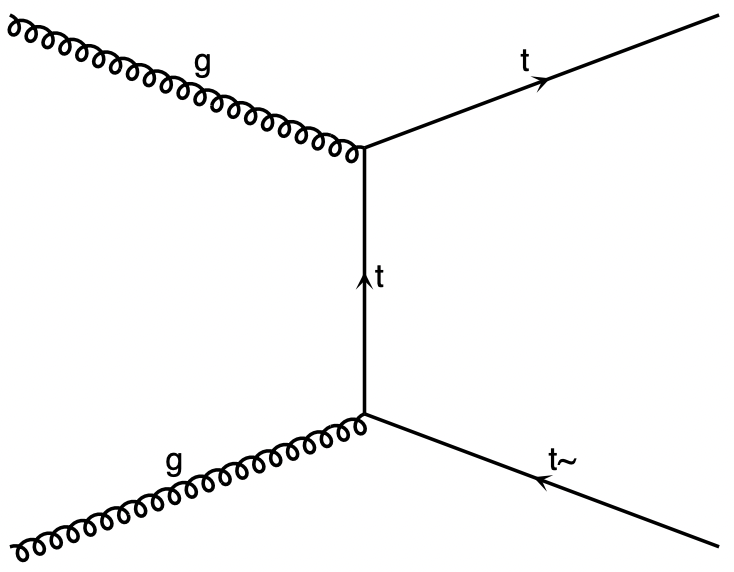
\includegraphics[width=\textwidth]{plots/ttbar.png}
\caption{$t\bar{t}$} \label{fig:ttbar}
\end{subfigure}
\begin{subfigure}[t]{0.3\textwidth}
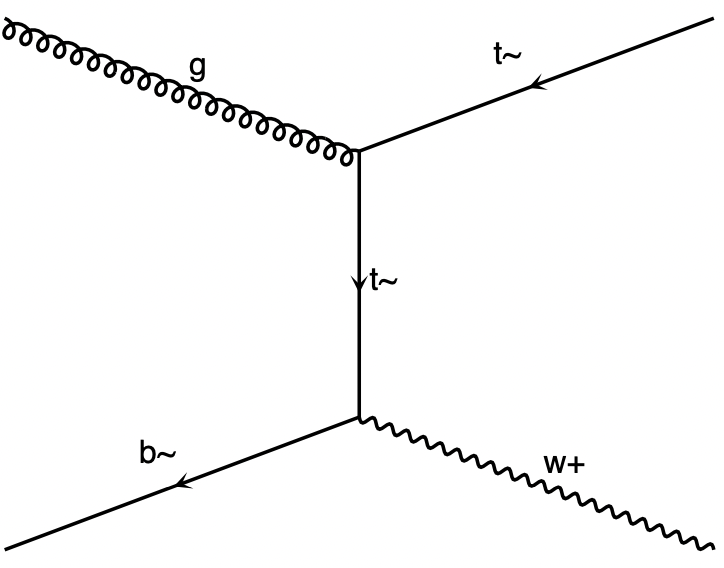
\includegraphics[width=\textwidth]{plots/tW.png}
\caption{$tW$} \label{fig:tW}
\end{subfigure}
\begin{subfigure}[t]{0.3\linewidth}
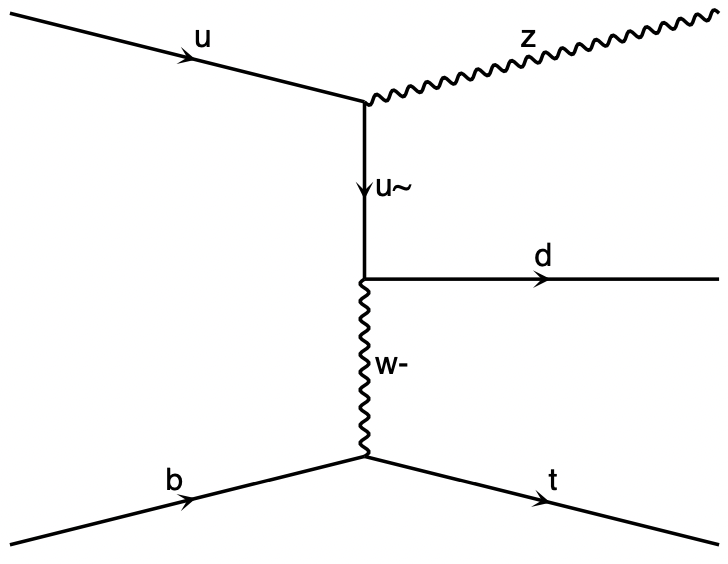
\includegraphics[width=\textwidth]{plots/tqz.png}
\caption{$tqZ$} \label{fig:tqz}
\end{subfigure}
\end{minipage}
\caption{Selected Feynman diagrams of $t\bar{t}$, $tW$ and $tqZ$}
\label{fig:feynman diagrams}
\end{figure}


In our study, we simulated three physics processes: top-antitop pair only ($t\Bar{t}$), a single (anti-)top quark in association with a $W$ boson ($tW$), and a single top in conjunction with a jet and a Z boson ($tqZ$). The event generation is carried out using \texttt{MadGraph5\_aMC@NLO} with Next-to-Leading Order (NLO) accuracy, incorporating MadSpin for the handling of particle decays with the following \texttt{MG5\_aMC} default parameters: 

\begin{align}
    &m_t=172.5 \, \GeV \\ &m_H=125 \, \GeV \\
    &m_W=80.399 \, \GeV \\ &m_Z=91.188 \, \GeV
\end{align}

The matrix element calculation with \texttt{MadGraph5\_aMC@NLO} simulates both $t\bar{t}$ and $tqZ$ processes with the model of \texttt{loop\_sm-no\_b\_mass}, which excludes the mass of the bottom quark for efficiency. The simulation employs a user-defined dynamical scale, $Q^2=m_t^2+0.5(p_t^2+p_{\bar{t}}^2)$, ensuring that the scale adapts based on the kinematics of the event. This scale allows for precise control over the factorization and renormalization scales.

In terms of the parton showering and hadronization with Pythia8, $t\bar{t}$ and $tqZ$ samples are configured with Parton Distribution Function (PDF) \texttt{A14 NNPDF23LO} set while $tW$ showers with \texttt{NNPDF30\_NLO} of version 2.3 PDF to model underlying event and fragmentation processes accurately. The Pythia8 settings include the anti-$k_t$ jet algorithm with a jet radius of 0.4 and a minimum jet $p_T$ threshold of 0.1 GeV, ensuring proper jet clustering and event topology.

Both $tW$ and $tqZ$ adopt the five-flavor scheme (5FS), where the bottom quark is treated as a massless parton in the initial state, enhancing computational efficiency while retaining NLO accuracy in top quark decays. Their $DSIS$ are 
$\texttt{525954}$ and $\texttt{950775}$ separately. This analysis is based on 5 million events with a center-of-mass energy of 13 TeV for all processes.

MadSpin setup is used for $t\bar{t}$ and $tqZ$ processes, for the decay of resonant particles, maintaining the spin correlations between the production and decay.

\section{Rivet Analysis}
The Rivet framework and the YODA\cite{buckley2024consistentmultidimensionaldifferentialhistogramming} histogram library are used to analyze and verify Monte Carlo event generators and samples using the above setups. The inclusive reductions on the negative weights fractions with NLO-$\Delta$ are analysed and shown with the unmodified Rivet routine, i.e., \texttt{MC\_XS}. Then, differential cross sections of the $t\Bar{t}$ process with various kinematics are compared between NLO with NLO-$\Delta$ in the framework of \texttt{MC\_TTBAR}. Last but not least, we compared MC samples, generated with both NLO and NLO-$\Delta$, with a set of experimental data to validate the correctness of the Monte Carlo simulation.



%%%%%%%%%%%%%%%%%% MC_XS %%%%%%%%%%%%%%%%%%%%%%
% 1. What's MC_XS for? What info it can provide?
% 2. Why do we need MC_XS?
% 3. How does MC_XS work?


To plot the distributions for the comparisons of NLO-$\Delta$ with NLO, a Python script using the YODA Python interface for loading and modifying the histograms is used. It loads a collection of YODA files as an update step, and then extracts the different systematic variations either from the weighted variation distributions in the nominal file, or from the nominal distributions of the systematic variation files, depending on the variation in question. Finally, the processed and reordered histograms are written as new YODA files, which are then plotted with the \texttt{rivet-mkhtml} Rivet tool.

For the evaluation of inclusive negative-weight fractions for all processes, a routine named \texttt{MC\_XS} within the Rivet framework has been used. The output of multiple grid jobs is combined into the numbers of negative-weight events or positive-weight events reported by \texttt{MC\_XS}. 

Regarding differential negative-weight fractions, the \texttt{MC\_TTBAR} Rivet routine is used to analyze the $t\Bar{t}$ process, characterizing the top-quark final-state via jet and lepton reconstruction rather than the unreliable partonic tops. The final states to be analysed can be selected via the \texttt{TTMODE} switch when running the routine. As a starting point of the analysis, the code of Rivet routine of the $t\Bar{t}$ cross-section measurement is used.  Due to the requirement of producing a MC Rivet routine, the detector-specific cuts on $|\eta|$ of the objects are opened up to $|\eta|>4.9$. In the routine, lepton refers to either $e$ or $\mu$. For the object selection, $e^\pm$ with $|\eta|<2.47$ and $p_T>7GeV$ and $\mu^\pm$ with $|\eta|<2.5$ and $p_T>6GeV$ are selected. The jets are defined by the anti-kT algorithm\cite{Cacciari_2008} with a radius parameter of $\Delta R=0.4$, and are required to have $|\eta|<2.5$ and $p_T>30GeV$.

Among different kinematics, we look into transverse momentum $p_T$ and the scalar sum of the transverse momentum
of all jets $H_T$ specifically.



%-------------------------------------------------------------------------------
\chapter{Results}
\label{chap:result}
%-------------------------------------------------------------------------------
\section{Inclusive reduction on NWF}
In this section we present MC@NLO-$\Delta$ predictions on inclusive and differential fractions of negative-weight events for three hadroproduction processes of $t\Bar{t}$, $tW$, and $tqZ$, and compare them with their MC@NLO counterparts. By comparing both MC@NLO-$\Delta$ and MC@NLO results with different datasets, we validate the correctness of MC modeling. Last but not least, we test the running time among different folding parameters with different descriptions. All of these results have been obtained by means of \texttt{MG5\_AMC} and \texttt{PYTHIA8} within the framework of AthGeneration 23.6.21.



\begin{table}[h!]
\centering
\begin{tabular}{||c| c c c | c c c||} 
 \hline
  & & MC@NLO & & & MC@NLO-$\Delta$ & \\ [0.5ex]
 \hline
  process & 111 & 221 & 441 & $\Delta$-111 & $\Delta$-221 & $\Delta$-441 \\ [0.5ex] 
  \hline
  $pp\rightarrow t\Bar{t}$ & $21.9\%$ & $19.3\%$ & $19.0\%$ & $8.8\%$ & $4.7\%$ & $4.2\%$ \\
  $pp\rightarrow tW$ & $18.7\%$ & $14.1\%$ & $13.3\%$ & $9.7\%$ & $4.0\%$ & $2.8\%$ \\ 
  $pp\rightarrow tqZ$ & $32.4\%$ & $24.8\%$ & $20.8\%$ & $34.4\%$ & $27.3\%$ & $24.5\%$ \\
 \hline
\end{tabular}
\caption{Fractions of negative-weight events for $t\Bar{t}$, $tW$ and $tqZ$ processes, computed with MC@NLO and with MC@NLO-$\Delta$, for three different choices of the folding parameters.}
\label{table:inclusive negative fraction}
\end{table}


% Details of doing the analysis, check the details of the code.
% What type of cuts have been used? pT cut, how to reconstruct the jet?


% Results of inclusive reductions on NWF
Table \ref{table:inclusive negative fraction} shows the overall fractions of negative-weight events for each process. For both $t\bar{t}$ and $tqZ$, switching to MC@NLO-$\Delta$ leads to a significant reduction in the fraction of negative-weight events compared to standard MC@NLO except for $tqZ$ process. For pp to $t\Bar{t}$ process, the reduction on NWF is up to $50\%$ or even more compared to the result offered in the paper\cite{NLO_matching}. The effect of increasing the folding parameters leads to fewer negative-weight fractions in both MC@NLO-$\Delta$ and MC@NLO descriptions. However, the $pp\rightarrow tqZ$ process remains particularly challenging. [offer some possible explanations?]


\section{Differential reduction on NWF}
%%%%%%%%%%% results of differential reductions on NWF %%%%%%%%%%%%%
We now turn to considering differential distributions. We point out that, for each process, we have studied the behaviour of dozens of observables, with the largest numbers in the cases of the processes with richer final states. For the sake of this analysis, in view of the limitations of space it entails, we have restricted ourselves to discussing the case of an observable which is very often used as a test case in the context of matching procedures, namely both $p_T$ and $H_T$.

As illustration, we now show for the $t\bar{t}$ process the differential distributions of the $p_T$ and $H_T$ observables, which are commonly used as a test case for matching procedures. The behaviour of many other observables were also studied and in general good agreement was observed between the delta maching and nominal MC setups.

\begin{figure}[t]
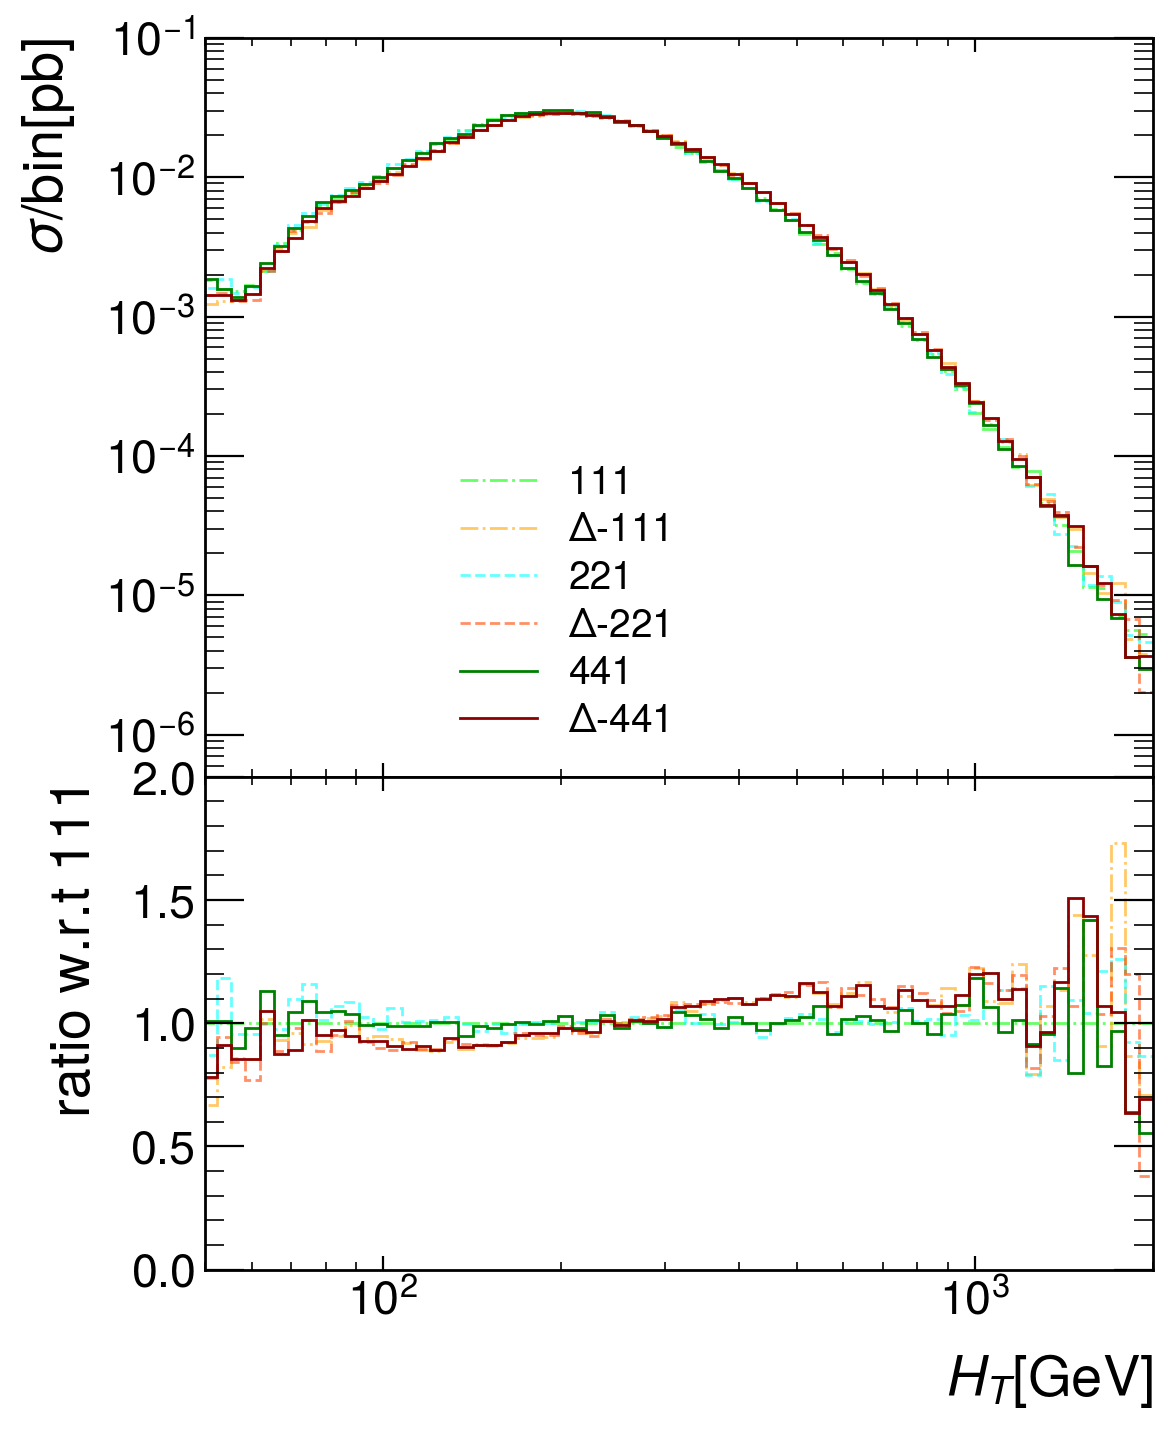
\includegraphics[width=8cm]{plots/NWF_ttbar_folding_HT.png}
\centering
\caption{the $H_T$ of the $t\Bar{t}$ process}
\end{figure}


\section{Validation of MC}
%%%%%%%%%%% Compare MC with Data %%%%%%%%%%%%%%%%

For the purpose of MC validation, we compare MC simulation results with experimental results from the following data sets downloaded from HepDATA: \texttt{ATLAS\_2017\_I1495243}\cite{ATLAS_2017_I1495243}, \texttt{ATLAS\_2018\_I1677498}\cite{ATLAS_2018_I1677498}, \texttt{ATLAS\_2019\_I1750330}\cite{ATLAS_2019_I1750330}, \texttt{ATLAS\_2019\_I1759875}\cite{ATLAS_2019_I1759875}, \texttt{CMS\_2018\_I1620050}\cite{CMS_2018_I1620050}, \texttt{CMS\_2022\_I2129461}\cite{CMS_2022_I2129461}. We first start by examining the comparison between MC with rivet analysis of \texttt{ATLAS\_2017\_I1495243}\cite{ATLAS:2017qjg} and measurements of jet activity in top-quark pair events produced in proton-proton collisions with 3.2 $fb^{-1}$ in 2017. Events are chosen by requiring an opposite-charge $e\mu$ pair and two $b$-tagged jets in the final state. The normalized differential cross-sections of top-quark pair production are presented as functions of additional-jet and the corresponding transverse momentum, $p_T$. For the object selection, $e^\pm$ and $\mu^\pm$ with $|\eta|<2.5$ and $p_T>25GeV$ are selected and dressed with photons in a cone of $\Delta R<0.1$. The jets are defined by the anti-kT algorithm with a radius parameter of $\Delta R=0.4$, and are required to have $|\eta|<2.5$ and $p_T>25GeV$. 

The comparison between data with MC simulation from both MC@NLO and MC@NLO-$\Delta$ is given by Figure \ref{fig:ATLAS_2017_leading_bjet_pT}. In the upper panel, the particle-level normalized cross-sections differential in jet $p_T$ is plotted as a function of $p_T$ of the leading b jet, where the data points are shown in blue, and NLO and NLO-$\Delta$ are depicted in red and green, respectively. Both $\Delta$ and without $\Delta$ prescriptions closely match the data, indicating that NLO-$\Delta$ captures the same physics underlying physics as the standard NLO. To further examine the agreement between simulations and data, the ratios of MC results to data are shown in the middle panel, with purple shaded areas representing data uncertainties. Both NLO and NLO-$\Delta$ fall within data uncertainty bands, highlighting their consistency with experimental measurements. The lower panel shows the ratio of NLO-$\Delta$ to NLO, showing that NLO-$\Delta$ introduces differences in the high $p_T$ region compared to NLO.


\begin{figure}[htp]
\centering
\begin{minipage}{\linewidth}
\begin{subfigure}[t]{0.45\textwidth}
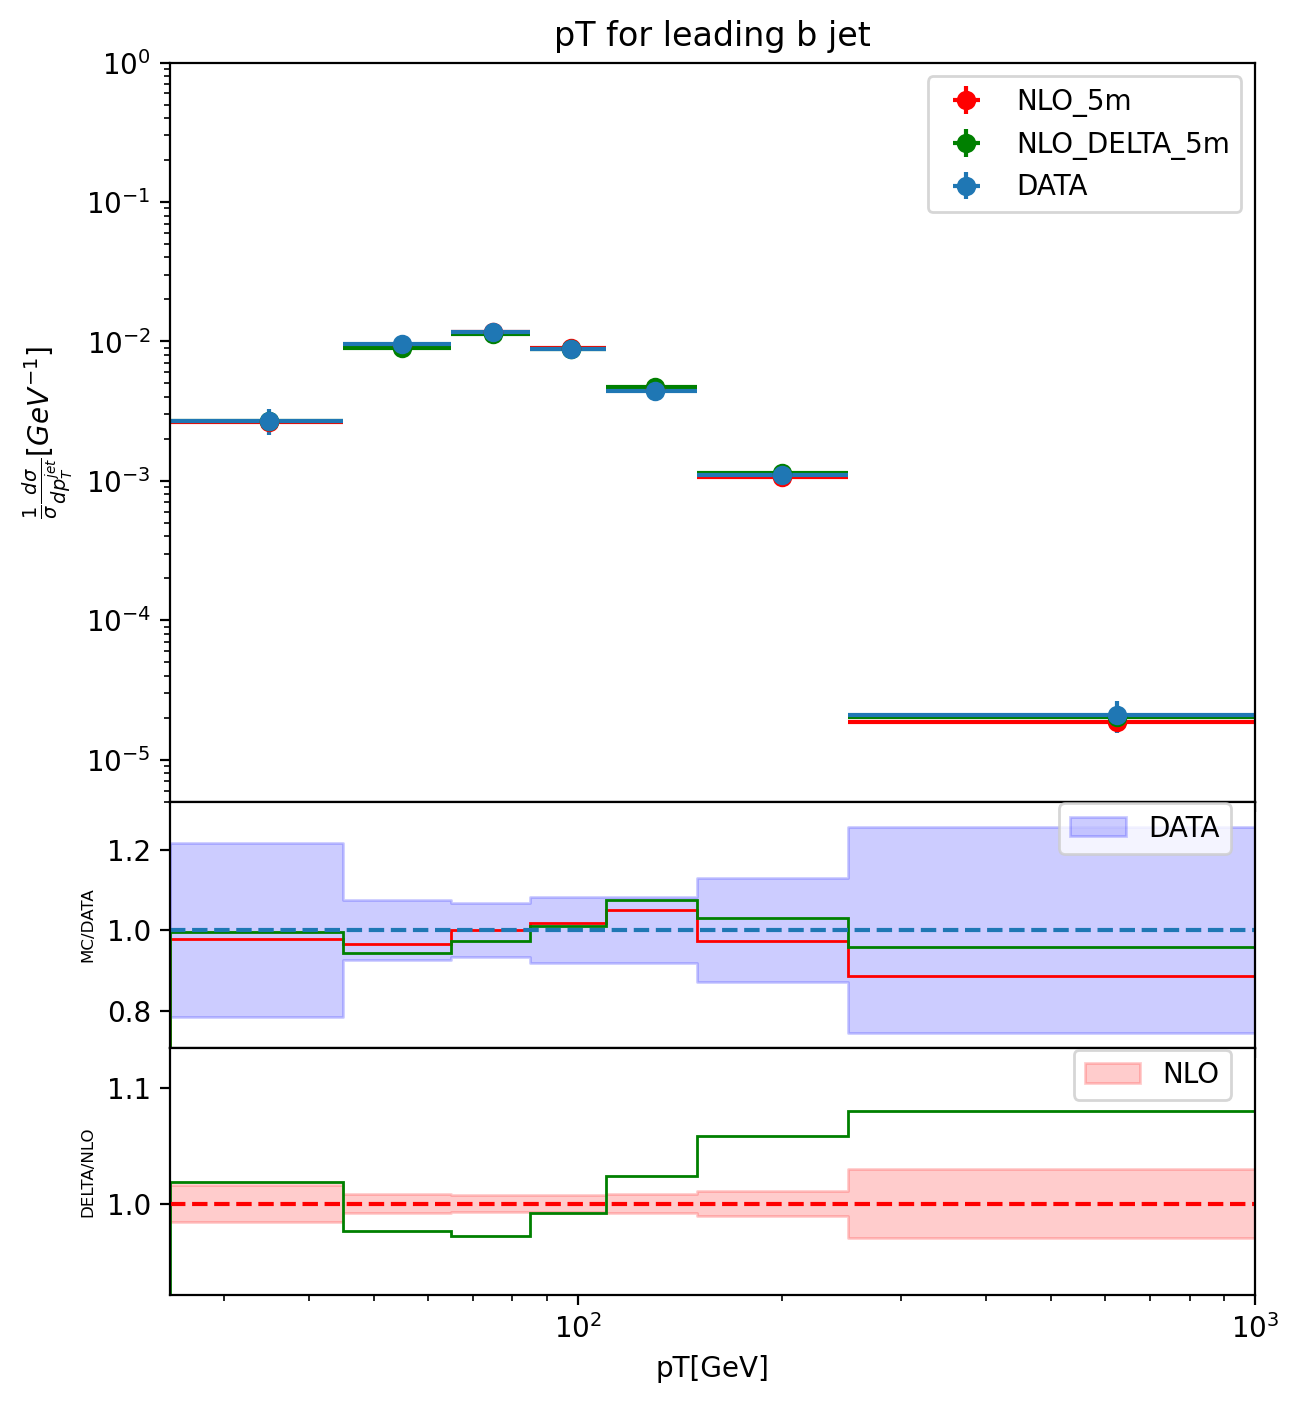
\includegraphics[width=\textwidth]{plots/ATLAS_2017_I1495243_lead_bjet_JO.png}
\caption{leading b jet $p_T$} \label{fig:ATLAS_2017_leading_bjet_pT}
\end{subfigure}
\begin{subfigure}[t]{0.5\textwidth}
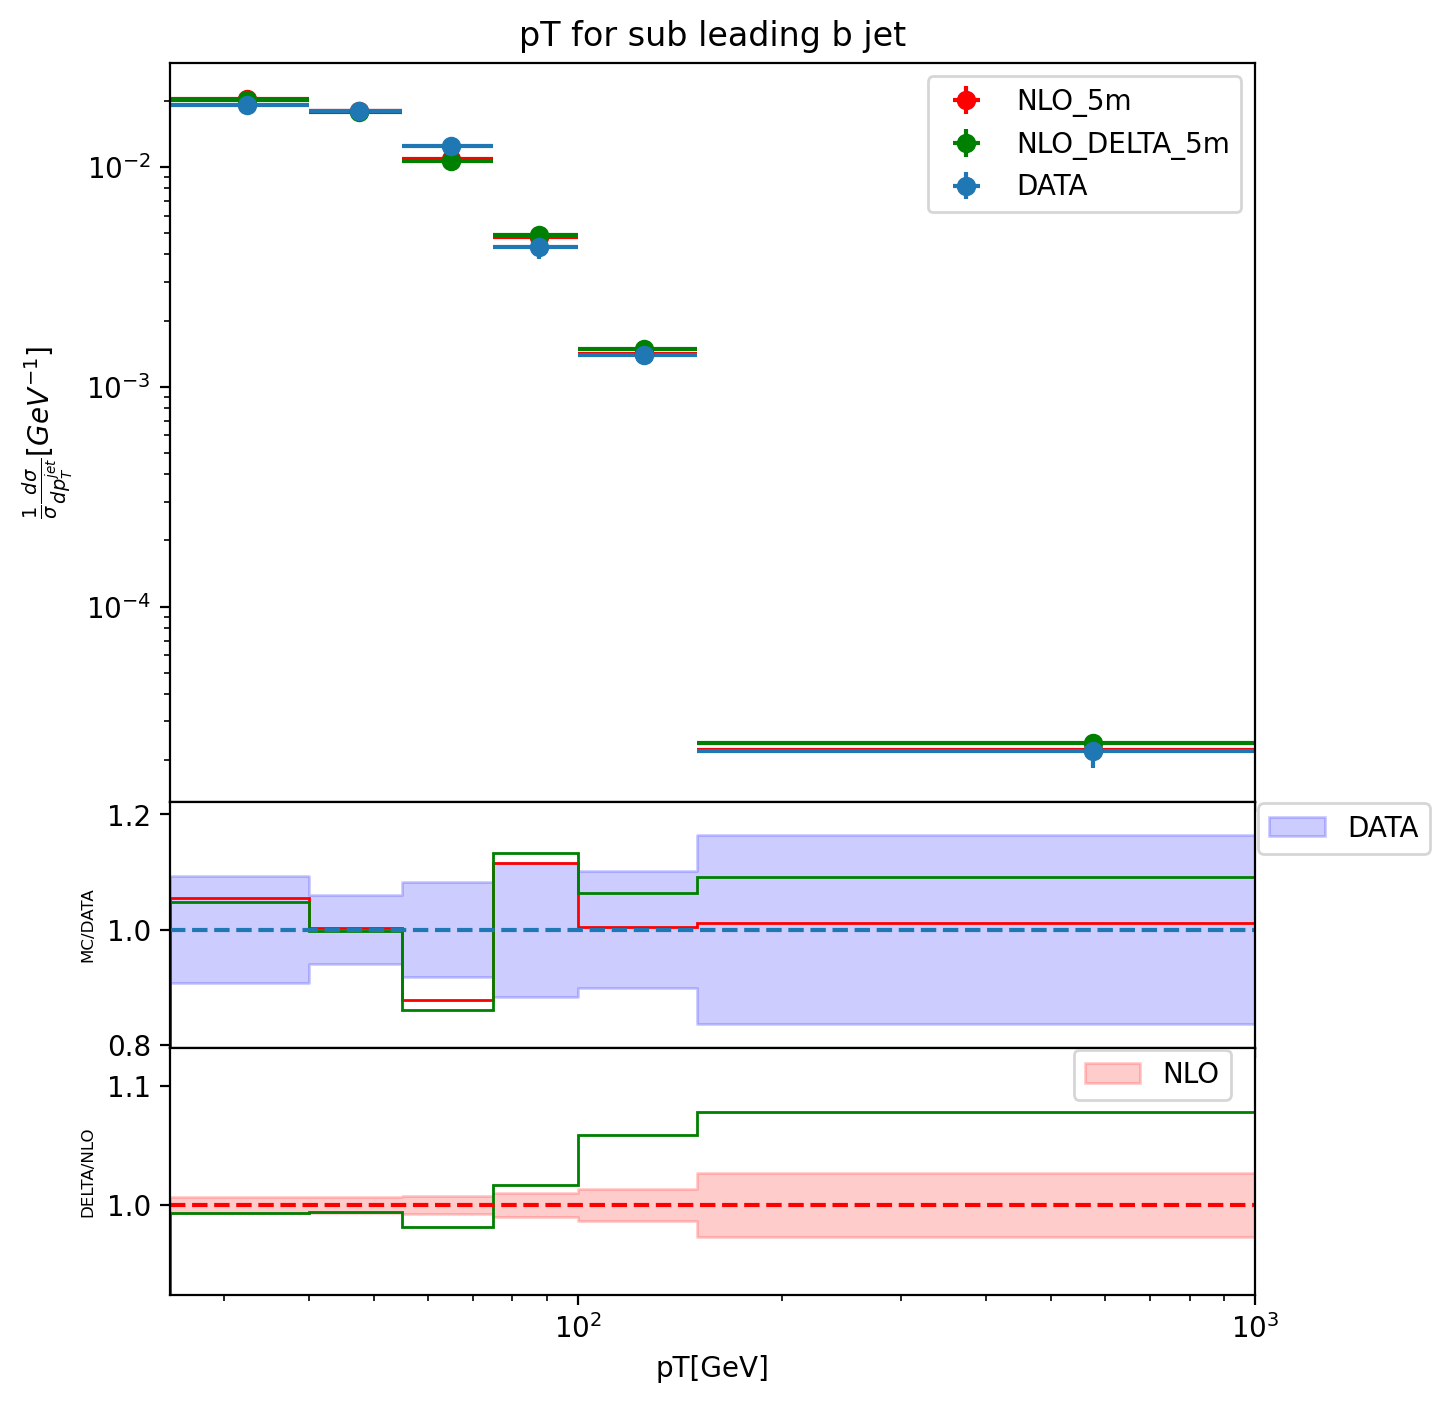
\includegraphics[width=\textwidth]{plots/ATLAS_2017_I1495243_sub_lead_bjet_JO.png}
\caption{subleading b jet $p_T$}
\label{fig:ATLAS_2017_subleading_bjet_pT}
\end{subfigure}
\end{minipage}
\caption{jet $p_T$ distribution for (a) leading b-jet, (b) sub-leading b-jet.  Comparison to MC predictions is shown for this distribution in the first panel. The middle and bottom panels show the ratios of different MC predictions of the normalized cross-section to the measurement and the ratios of MadGraph5+Pythia8 predictions with variation of the QCD radiation to the measurement, respectively. The shaded regions show the statistical uncertainty for data (purple) and for MG5@NLO (red)}
\label{fig:ATLAS_2017_lead&subleading_bjet_pT}
\end{figure}




\section{Running time Comparison}
%%%%%%%%%%% results of running time %%%%%%%%%%%%%%%%%%

% 1. what type of configuration you use to run it? Wall time? SLAC? CPU? 
% 2. 

Now we aim to discuss the computational time required for different processes. It is crucial to ensure that the runtime associated with the NLO-$\Delta$ matching configuration does not significantly exceed that of the standard NLO configuration. Otherwise, it would not be computationally efficient to allocate resources to the NLO-$\Delta$ configuration. Batch jobs are submitted for Monte Carlo event generation using ATLAS software on a High-Performance Computing (HPC) cluster managed by Slurm. To cover the memory requirement for all jobs, the minimum memory allocated
48 per worker node is set to 8 GB in the job submission. This restricts the available resources on which the
100 jobs can run to special high-memory worker nodes on SLAC Shared Scientific Data Facility (S3DF) with 48 CPU cores. The detailed environment configuration and job parameters are attached to the Appendix. According to Table \ref{table:computational time}, NLO-$\Delta$ configuration demonstrates comparable or slightly similar performance to NLO matching across three cases, with relative difference remaining below 10\%. 


\begin{table}[h!]
\centering
\begin{tabular}{||c| c c c | c c c||} 
 \hline
  & & MC@NLO & & & MC@NLO-$\Delta$ & \\ [0.5ex]
 \hline
  process & 111 & 221 & 441 & $\Delta$-111 & $\Delta$-221 & $\Delta$-441 \\ [0.5ex] 
  \hline
  $pp\rightarrow t\Bar{t}$ & 3150s & 3168s & 3166s & 3096s & 3069s & 3134s \\
  $pp\rightarrow tW$ & 2420s & 2083s & 2173s & 2422s & 2404s & 2638s \\ 
  $pp\rightarrow tqZ$ & 2560s & 2776s & 2771s & 2550s & 2758s & 2690s \\
 \hline
\end{tabular}
\caption{Fractions of negative-weight events for $t\Bar{t}$, tW and tqZ processes, computed with MC@NLO and with MC@NLO-$\Delta$, for three different choices of the folding parameters.}
\label{table:computational time}
\end{table}

However, it's worth noticing that the tqZ process, particularly when employing gridpack integration, necessitates additional pre-running time due to the complexity of the events and the large number of diagrams compared to a tree-level process involved. The computing times for the gridpack integration of the tqZ process under different configurations are summarized in Table \ref{table:gridpack time}. Notably, the NLO-$\Delta$ configuration consistently requires more computational time compared to their NLO counterparts, with the time escalating as the folding parameters increase. On the other hand, for the tqZ process under different folding parameters, the gridpack integration times reflect the substantial computational demand. For example, the integration time for the 441 configuration for NLO and NLO-$\Delta$ reach up to 75 hours and 97 separately. This marked increase is indicative of the growing computational complexity as the folding parameters are increased.

\begin{table}[h!]
\centering
\begin{tabular}{||c| c c c | c c c||} 
 \hline
  & & MC@NLO & & & MC@NLO-$\Delta$ & \\ [0.5ex]
 \hline
  process & 111 & 221 & 441 & $\Delta$-111 & $\Delta$-221 & $\Delta$-441 \\ [0.5ex] 
 \hline
  $pp\rightarrow tqZ$ & 7 hrs & 21 hrs & 75 hrs & 11 hrs & 28 hrs & 97 hrs \\
 \hline
\end{tabular}
\caption{Computing time of gridpack integration for tqZ processes, computed with MC@NLO and with MC@NLO-$\Delta$, for three different choices of the folding parameters.}
\label{table:gridpack time}
\end{table}

Overall, while the NLO-$\Delta$ setup introduces a new matching configuration, its efficiency in terms of computing time remains closely aligned with that of the regular NLO approach, maintaining a manageable overhead. This similarity suggests that adopting the NLO-$\Delta$ configuration may not significantly compromise computational efficiency, making it a viable option for simulations that require this matching scheme.

\chapter{Conclusion}
\label{chap:discussion}
%-------------------------------------------------------------------------------

Combining the information above
\clearpage


\chapter*{Appendix}
%"mystyle" code listing set
\lstset{style=mystyle}

\begin{lstlisting}[language=Python, caption=Job Configuration python script]
from datetime import datetime
import shutil
import os
import ROOT

walltime="7100"
numOfEventsPerJob=5000
numOfJobs=1
ncores=48

# JOs path
JO_name = 'mc.MGPy8EG_ttbar_NLO_fold_111.py'
jobOpt = "/fs/ddn/sdf/group/ldmx/users/dongyi/data/JO/100000/%s" % JO_name

# Output container
output_dir = "/fs/ddn/sdf/group/ldmx/users/dongyi/data/BATCH/Output_JO/test_1"

#tar_ball = "/fs/ddn/sdf/group/ldmx/users/dongyi/data/BATCH/Output_JO/integration_tqz_NLO_5FS_221/output/job_0/999999/mc_13TeV.MGPy8EG_tllq_5FS_HT6_NLO_211.GRID.tar.gz"

# ===========================================
#             GENERATE COMMAND
# ===========================================


def batch_cmd(fileName,job_output,payload):

  runscript = open(fileName, 'a+')
  runscript.write("#!/bin/bash \n \n")
  runscript.write("#BSUB -W%s \n \n" % walltime)

  runscript.write("#SBATCH --account=atlas:usatlas \n")
  runscript.write("#SBATCH --partition=roma \n")
  runscript.write("#SBATCH --job-name=job_0 \n" )
  runscript.write("#SBATCH --output=%s/output.log \n" % job_output)
  runscript.write("#SBATCH --error=%s/error.log \n" % job_output)
  runscript.write("#SBATCH --ntasks=1")
  runscript.write("#SBATCH --nodes=1")
  runscript.write("#SBATCH --cpus-per-task=%i \n" % ncores)
  runscript.write("#SBATCH --mem-per-cpu=8g \n")
  runscript.write("#SBATCH --time=0-04:00:00 \n \n") 
  
  runscript.write("export ATLAS_LOCAL_ROOT_BASE=/cvmfs/atlas.cern.ch/repo/ATLASLocalRootBase \n")
  runscript.write("export ALRB_CONT_CMDOPTS='-B /sdf,/fs,/cvmfs' \n")
  runscript.write("export ALRB_CONT_RUNPAYLOAD='source %s' \n" % payload)
  runscript.write("source $ATLAS_LOCAL_ROOT_BASE/user/atlasLocalSetup.sh -c centos7 \n")

  runscript.close()

def payload_cmd(fileName, job_index, job_output, randomSeed):
  
  runscript = open(fileName, 'a+')
  
  runscript.write("source ~/.bashrc \n")
  runscript.write("asetup AthGeneration 23.6.21 \n")
  runscript.write("source setupRivet \n")
  runscript.write("cd /fs/ddn/sdf/group/ldmx/users/dongyi/data/NWF \n")

  runscript.write("cd %s \n" % job_output)
  runscript.write("\n \n")

  # Use multiple cores for event generation!
  runscript.write("export ATHENA_PROC_NUMBER=%i \n" % ncores )
  #runscript.write("\n \n")

  # Link to rivet
  runscript.write("export RIVET_DATA_PATH=/cvmfs/atlas.cern.ch/repo/sw/software/23.6/sw/lcg/releases/MCGenerators/rivet/4.0.0-39772/x86_64-centos7-gcc11-opt/share/Rivet:/fs/ddn/sdf/group/ldmx/users/dongyi/data/key_files/data_samples/CMS_2022_I2129461 \n")
  runscript.write("export RIVET_ANALYSIS_PATH=/cvmfs/atlas.cern.ch/repo/sw/software/23.6/sw/lcg/releases/MCGenerators/rivet/4.0.0-39772/x86_64-centos7-gcc11-opt/lib/Rivet:/fs/ddn/sdf/group/ldmx/users/dongyi/data/NWF:/fs/ddn/sdf/group/ldmx/users/dongyi/data/key_files/data_samples/CMS_2022_I2129461/ \n")

  runscript.write("asetup AthGeneration 23.6.21 \n \n")
  # Build up transform
  runscript.write("Gen_tf.py --ecmEnergy=13000 \\\n" )
  runscript.write("\t\t--firstEvent=1 \\\n")
  runscript.write("\t\t--maxEvents=%i  \\\n" % numOfEventsPerJob )
  runscript.write("\t\t--randomSeed=%i \\\n" %randomSeed)
  runscript.write("\t\t--generatorJobNumber=999999 \\\n")
  runscript.write("\t\t--jobConfig=%s \\\n" % job_output)
  #runscript.write("\t\t--postInclude=/fs/ddn/sdf/group/ldmx/users/dongyi/data/BATCH/JO.py \\\n")
  runscript.write("\t\t--outputEVNTFile=output.EVNT.%i.root \\\n" % job_index )
  runscript.write("\n \n")
  #runscript.write("rm -rf %s/*.root* " % job_output )

  runscript.close()

def getScriptFolder():

  # Master location
  script_dir=output_dir+'/scripts/'

  # Get the scripts directory that was used
  # in a different submission
  script_dir = script_dir+str(datetime.now().strftime('%Y-%m-%d_%H-%M-%S'))
  if not os.path.exists(script_dir):
    os.makedirs(script_dir)

  return script_dir

# ===========================================
#         SUBMISSION COMMAND
# ===========================================

# Make the output directory if it
# doesn't already exist
if not os.path.exists(output_dir+'/output/'):
  os.makedirs(output_dir+'/output/')

# Store generated scripts into a folder
# indexed by the year-month-day
script_folder=getScriptFolder()
nResubmissions=0

# Random number generator
rn = ROOT.TRandom()

job=0

# Loop over samples
for j in range(0,numOfJobs) :

  print('Submitting jobs number %s ' % j )

  # Generated script and job output 
  bsub_script = "%s/batch_script_job%i.sh" % (script_folder,j)
  payload_script= "%s/payload_script_job%i.sh" % (script_folder,j)
  job_output  = '%s/output/job_%i/999999/' % (output_dir,j)
  #slurm_job   = "%s/job_%i" % (slurm_folder,j)

  #
  if not os.path.exists(job_output):
    os.makedirs(job_output)

  rndm = rn.Integer(100000)

  # Generate the submission script
  payload_cmd(payload_script,j,job_output,rndm)
  batch_cmd(bsub_script,job_output,payload_script)

  os.symlink(jobOpt,'%s/%s' % (job_output, JO_name) )
  #os.symlink(tar_ball,'%s/mc_13TeV.MGPy8EG_tllq_5FS_HT6_NLO_221.GRID.tar.gz' % (job_output))

  #SlurmJob(slurm_job, bsub_script, job_output)

  cmd = "sbatch  "
  cmd += " %s " % bsub_script
 
  print(cmd)
  os.system(cmd)

\end{lstlisting}
\clearpage

\begin{lstlisting}[language=python, caption=$t\bar{t}$ job option python script]
from MadGraphControl.MadGraphUtils import *
from MadGraphControl.MadGraphParamHelpers import set_top_params
import MadGraphControl.MadGraph_NNPDF30NLO_Base_Fragment

import fileinput


# Make some excess of events - make sure we protect against maxEvents=-1
evgenConfig.nEventsPerJob = 10000
nevents=1.1*runArgs.maxEvents if runArgs.maxEvents>0 else 1.1*evgenConfig.nEventsPerJob


process="""
import model loop_sm-no_b_mass
define p = g u c d s u~ c~ d~ s~ b b~
define j = g u c d s u~ c~ d~ s~ b b~
generate p p > t t~ [QCD]
output -f"""

process_dir = new_process(process)

#Fetch default NLO run_card.dat and set parameters
settings = {'parton_shower' : 'PYTHIA8',
            'folding' : '2, 2, 1', # Here's the knob to set the folding parameters
            'mcatnlo_delta' : 'True', # This is the MC@NLO-Delta switch to turn it on
            'maxjetflavor'  : 5,
            'dynamical_scale_choice' : '10', #user-defined scale -> Dominic's definition of mt+1/2*(pt^2+ptx^2)
            'jetalgo'   : '-1',  # use anti-kT jet algorithm
            'jetradius' : '0.4', # set jet cone size of 0.4
            'ptj'	: '0.1', # minimum jet pT
            'req_acc'   : '0.001',
            'bwcutoff'  : '50',
            'nevents':int(nevents)            
}


modify_run_card(process_dir=process_dir,runArgs=runArgs,settings=settings)
modify_config_card(process_dir=process_dir,settings={'pythia8_path':'/cvmfs/atlas.cern.ch/repo/sw/software/23.6/sw/lcg/releases/MCGenerators/pythia8/309-bb414/x86_64-centos7-gcc11-opt/'})
# Modify the param card
set_top_params(process_dir,mTop=172.5,FourFS=False)


# Cook the setscales file for the user defined dynamical scale
fileN = process_dir+'/SubProcesses/setscales.f'
mark  = '      elseif(dynamical_scale_choice.eq.10.or.dynamical_scale_choice.eq.0) then'
rmLines = ['ccccccccccccccccccccccccccccccccccccccccccccccccccccccccccccccccccccccccccccccccccc',
           'cc      USER-DEFINED SCALE: ENTER YOUR CODE HERE                                 cc',
           'cc      to use this code you must set                                            cc',
           'cc                 dynamical_scale_choice = 0                                    cc',
           'cc      in the run_card (run_card.dat)                                           cc',
           'write(*,*) "User-defined scale not set"',
           'stop 1',
           'temp_scale_id=\'User-defined dynamical scale\' ! use a meaningful string',
           'tmp = 0',
           'cc      USER-DEFINED SCALE: END OF USER CODE                                     cc'
           ]

for line in fileinput.input(fileN, inplace=1):
    toKeep = True
    for rmLine in rmLines:
        if line.find(rmLine) >= 0:
           toKeep = False
           break
    if toKeep:
        print(line),
    if line.startswith(mark):
        print("""
c         Q^2= mt^2 + 0.5*(pt^2+ptbar^2)
          xm2=dot(pp(0,3),pp(0,3))
          tmp=sqrt(xm2+0.5*(pt(pp(0,3))**2+pt(pp(0,4))**2))
          temp_scale_id='mt**2 + 0.5*(pt**2+ptbar**2)'
              """)


### Decay with MadSpin
madspin_card_loc=process_dir + '/Cards/madspin_card.dat'
mscard = open(madspin_card_loc,'w')
mscard.write("""#************************************************************
#*                        MadSpin                           *
#*                                                          *
#*    P. Artoisenet, R. Frederix, R. Rietkerk, O. Mattelaer *
#*                                                          *
#*    Part of the MadGraph5_aMC@NLO Framework:              *
#*    The MadGraph5_aMC@NLO Development Team - Find us at   *
#*    https://server06.fynu.ucl.ac.be/projects/madgraph     *
#*                                                          *
#************************************************************
# set Nevents_for_max_weight 250 # number of events for the estimate of the max. weight
# set max_weight_ps_point 1000  # number of PS to estimate the maximum for each event
 set BW_cut 50
 set seed %i
 define j = g u c d s b u~ c~ d~ s~ b~
 define l+ = e+ mu+ ta+
 define l- = e- mu- ta-
 define vl = ve vm vt
 define vl~ = ve~ vm~ vt~
 decay t > w+ b, w+ > l+ vl
 decay t~ > w- b~, w- > l- vl~
 launch
"""%(runArgs.randomSeed))
mscard.close()


generate(process_dir=process_dir,runArgs=runArgs)
arrange_output(process_dir=process_dir,runArgs=runArgs,lhe_version=3,saveProcDir=False)  

#--------------------------------------------------------------
# Pythia8 showering
#--------------------------------------------------------------
### Shower

include("Pythia8_i/Pythia8_A14_NNPDF23LO_EvtGen_Common.py")
include("Pythia8_i/Pythia8_aMcAtNlo.py")
include("Pythia8_i/Pythia8_ShowerWeights.py")


### Metadata
evgenConfig.description = 'MG5_aMC@NLO+MadSpin+Pythia8+EvtGen ttbar'
evgenConfig.generators    = ['MadGraph', 'Pythia8', 'EvtGen']
evgenConfig.keywords+=['ttbar','jets']
evgenConfig.contact  = ["jens.roggel@cern.ch" ]
\end{lstlisting}

\clearpage

\begin{lstlisting}[language=python, caption=$tW$ job option python script]
from MadGraphControl.MadGraphUtils import * 
from MadGraphControl.MadGraphParamHelpers import set_top_params
from MadGraphControl.DiagramRemoval import do_DRX
import MadGraphControl.MadGraph_NNPDF30NLO_Base_Fragment

evgenConfig.nEventsPerJob = 5000
nevents = int(1.2*runArgs.maxEvents) if runArgs.maxEvents > 0 else int(1.2*evgenConfig.nEventsPerJob)


DR_mode=1

tandw_decays = """
decay t > w+ b, w+ > l+ v
decay t~ > w- b~, w- > l- v~
decay w+ > l+ v
decay w- > l- v~
"""



gen_process = """
import model loop_sm-no_b_mass
define p = g u c d s b u~ c~ d~ s~ b~
define j = g u c d s b u~ c~ d~ s~ b~
define w = w+ w-
define ttbar = t t~
generate p p > ttbar w [QCD]
output -f
"""
process_dir = new_process(gen_process)

set_top_params(process_dir,mTop=172.5,FourFS=False)



#Call DR code
do_DRX(DR_mode,process_dir)
    
run_settings = { 
    'nevents'    : nevents,
    'folding'    : '2, 2, 1',
    'lhe_version':'3.0',
    'mcatnlo_delta' : 'True',
    'maxjetflavor'  : 5,
    'parton_shower' : 'PYTHIA8',
    'fixed_ren_scale' : "False",
    'fixed_fac_scale' : "False",
    'fixed_QES_scale' : "False",
    'mll_sf'        : -1,
    'req_acc' :0.001,
}

# Set up the process

# Set up the run card
modify_run_card(process_dir=process_dir,runArgs=runArgs,settings=run_settings)
modify_config_card(process_dir=process_dir,settings={'pythia8_path':'/cvmfs/atlas.cern.ch/repo/sw/software/23.6/sw/lcg/releases/MCGenerators/pythia8/309-bb414/x86_64-centos7-gcc11-opt/'})
madspin_card_loc=process_dir+'/Cards/madspin_card.dat'                                                                                                                                   
mscard = open(madspin_card_loc,'w')  
mscard.write("""
  set max_weight_ps_point 500
  set BW_cut 50
 set seed {}
 # specify the decay for the final state particles
 define q = u d s c b
 define q~ = u~ d~ s~ c~ b~
 define l+ = e+ mu+ ta+
 define l- = e- mu- ta-
 define v = ve vm vt
 define v~ = ve~ vm~ vt~
 {}
 # running the actual code
 launch""".format(runArgs.randomSeed,tandw_decays))
mscard.close()


# Generate the events
generate(process_dir=process_dir,runArgs=runArgs)

# Remember to set saveProcDir to FALSE before sending for production!!
outputDS=arrange_output(process_dir=process_dir,runArgs=runArgs,lhe_version=3,saveProcDir=False)


#### Shower
## run Pythia8 on-the-fly -----------------------------------------------------
## Provide config information
evgenConfig.generators += ["aMcAtNlo", "Pythia8"]
evgenConfig.description = "MG5aMCatNLO/MadSpin/Pythia8"
evgenConfig.keywords    = ["SM","top"]
evgenConfig.contact     = ["andrej.saibel@cern.ch"]

include("Pythia8_i/Pythia8_A14_NNPDF23LO_EvtGen_Common.py")
## Enable MG5_aMC@NLO LHEF reading in Pythia8
include("Pythia8_i/Pythia8_LHEF.py")
#evgenConfig.generators += ["aMcAtNlo"]

#aMC@NLO default Pythia8 settings from http://amcatnlo.web.cern.ch/amcatnlo/list_detailed2.htm#showersettings
#plus MEC fix see https://arxiv.org/pdf/2308.06389.pdf
genSeq.Pythia8.Commands += ["SpaceShower:pTmaxMatch = 1",
                            "SpaceShower:pTmaxFudge = 1",
                            "SpaceShower:MEcorrections = off",
                            "TimeShower:pTmaxMatch = 1",
                            "TimeShower:pTmaxFudge = 1",
                            "TimeShower:MEcorrections = on",
                            "TimeShower:MEextended    = off",
                            "TimeShower:globalRecoil = on",
                            "TimeShower:limitPTmaxGlobal = on",
                            "TimeShower:nMaxGlobalRecoil = 1",
                            "TimeShower:globalRecoilMode = 2",
                            "TimeShower:nMaxGlobalBranch = 1.",
                            "TimeShower:weightGluonToQuark=1.",
                            "Check:epTolErr = 1e-2" ]
\end{lstlisting}

\clearpage

\begin{lstlisting}[language=python, caption=$tqZ$ job option python script]
from MadGraphControl.MadGraphUtils import *
from MadGraphControl.MadGraphParamHelpers import set_top_params
from MadGraphControl.MadGraph_NNPDF30NLOnf4_Base_Fragment import *

import fileinput

nevents = int(1.1*runArgs.maxEvents) if runArgs.maxEvents > 0 else int(1.1*evgenConfig.nEventsPerJob)

process = '''
import model loop_qcd_qed_sm
define l+ = e+ mu+ ta+
define l- = e- mu- ta-
set nlo_mixed_expansion False
generate p p > t j z $$ h [QCD] 
output -f
'''


process_dir = new_process(process)

# Write the run_card
settings = {
    'nevents':        nevents,
    'parton_shower':  "PYTHIA8",
    'folding'    : '2, 2, 1',
    'mcatnlo_delta' : 'True',
    'bwcutoff':50,
    'ptgmin':         20,
    'mll_sf':         5,
    'dynamical_scale_choice' : 10,
}


print("CUSTOM SCALE SETTINGS: SET TO HT/6")
dyn_scale_fact = 1.0
fileN = process_dir+'/SubProcesses/setscales.f'
mark = '      elseif(dynamical_scale_choice.eq.10.or.dynamical_scale_choice.eq.0) then'
rmLines = ['ccccccccccccccccccccccccccccccccccccccccccccccccccccccccccccccccccccccccccccccccccc',
           'cc      USER-DEFINED SCALE: ENTER YOUR CODE HERE                                 cc',
           'cc      to use this code you must set                                            cc',
           'cc                 dynamical_scale_choice = 10                                   cc',
           'cc      in the run_card (run_card.dat)                                           cc',
           'ccccccccccccccccccccccccccccccccccccccccccccccccccccccccccccccccccccccccccccccccccc',
           '        write(*,*) "User-defined scale not set"',
           '        stop 1',
           '        temp_scale_id=\'User-defined dynamical scale\' ! use a meaningful string',
           '        tmp = 0d0']
flag=0
for line in fileinput.input(fileN, inplace=1):
    toKeep = True
    for rmLine in rmLines:
        if line.find(rmLine) >= 0:
            toKeep = False
            break
    if toKeep:
        print(line),
    if line.startswith(mark) and flag==0:
        flag +=1
        print("""
c         sum of the transverse mass divide by 6
c         m^2+pt^2=p(0)^2-p(3)^2=(p(0)+p(3))*(p(0)-p(3))
          tmp=0d0
          do i=3,nexternal
            if ( (idup(i,1) .ge. 5) .or. (idup(i,1) .le. -5) ) then
              tmp=tmp+dsqrt(max(0d0,(pp(0,i)+pp(3,i))*(pp(0,i)-pp(3,i))))
            endif
          enddo
          tmp=tmp/6d0
          temp_scale_id='H_T/6 := sum_i mT(i)/6, i=t,H,b'
        """)
    if line.startswith("      common/ctemp_scale_id/temp_scale_id"):
        print("""
           integer idup(nexternal,maxproc)
           common /c_leshouche_inc/idup
        """)


modify_run_card(process_dir=process_dir, runArgs=runArgs, settings=settings)



param_card_settings = {
        'mass' : {
            '5':  "0.00000",
            '6':  "172.5",
            '15': "0",
            '23': "9.118760e+01",
            '24': "8.039900e+01",
            '25': "1.250000e+02",
                    },
        'yukawa' : { '6': "1.725000e+02 # ymt" },
        'DECAY' : {
            '5'  : """DECAY  5   0.000000e+00""",
            '15' : """DECAY  15   0.000000e+00""",
            '23' : """DECAY  23   2.495200e+00""",
            '24': """DECAY  24   2.085000e+00
                3.377000e-01   2   -1   2
                3.377000e-01   2   -3   4
                1.082000e-01   2  -11  12
                1.082000e-01   2  -13  14
                1.082000e-01   2  -15  16""",
                   }
        }

modify_param_card(process_dir=process_dir,params=param_card_settings)
modify_config_card(process_dir=process_dir,settings={'pythia8_path':os.getenv("PY8PATH")})

# Write the MadSpin card
madspin_card = process_dir+'/Cards/madspin_card.dat'
if os.access(madspin_card,os.R_OK):
    os.unlink(madspin_card)
mscard = open(madspin_card,'w')
mscard.write("""#************************************************************
#*                        MadSpin                           *
#*                                                          *
#*    P. Artoisenet, R. Frederix, R. Rietkerk, O. Mattelaer *
#*                                                          *
#*    Part of the MadGraph5_aMC@NLO Framework:              *
#*    The MadGraph5_aMC@NLO Development Team - Find us at   *
#*    https://server06.fynu.ucl.ac.be/projects/madgraph     *
#*                                                          *
#************************************************************
#Some options (uncomment to apply)
#
set seed %i
set Nevents_for_max_weight 75 # number of events for the estimate of the max. weight
set BW_cut 50                 # cut on how far the particle can be off-shell
set max_weight_ps_point 400   # number of PS to estimate the maximum for each event
# specify the decay for the final state particles
define l+ = e+ mu+ ta+
define l- = e- mu- ta-
define vl = ve vm vt
define vl~ = ve~ vm~ vt~
decay t > w+ b, w+ > l+ vl
decay t~ > w- b~, w- > l- vl~
# running the actual code
launch"""%(runArgs.randomSeed))
mscard.close()


# Print and generate
print_cards()
generate(process_dir=process_dir,
         grid_pack=True,
         gridpack_compile=False,
         required_accuracy=0.0005,
         runArgs=runArgs)
outputDS = arrange_output(process_dir=process_dir,
                          runArgs=runArgs,
                          saveProcDir=False,
                          lhe_version=3)


#### Shower: Py8 with A14 Tune and new MEC
include("Pythia8_i/Pythia8_A14_NNPDF23LO_EvtGen_Common.py")
include("Pythia8_i/Pythia8_aMcAtNlo_decayMEC.py")
include("Pythia8_i/Pythia8_ShowerWeights.py")


# Metadata
evgenConfig.description      = 'aMcAtNlo_tllq with HT/6 scale and new MEC'
evgenConfig.keywords        += ['SM','tZ']
evgenConfig.contact          = ['dominic.hirschbuehl@cern.ch']
evgenConfig.generators       = ['aMcAtNlo']
\end{lstlisting}

%-------------------------------------------------------------------------------
% If you use biblatex and either biber or bibtex to process the bibliography
% just say \printbibliography here.
\printbibliography
% If you want to use the traditional BibTeX you need to use the syntax below.
% \bibliographystyle{obsolete/bst/atlasBibStyleWoTitle}
% \bibliography{mydocument,bib/ATLAS,bib/CMS,bib/ConfNotes,bib/PubNotes}
%-------------------------------------------------------------------------------


%-------------------------------------------------------------------------------
% Extra tables etc. for HepData - comment in the following line if you have any.
% \section{HepData material}
%-------------------------------------------------------------------------------

This file is available for detailed tables etc.\ that are going to be
submitted to HepData or other similar destinations.
%-------------------------------------------------------------------------------

\end{document}
